\documentclass[14pt]{extreport}
\usepackage[utf8]{inputenc}
\usepackage[german]{babel}
\usepackage{wrapfig}
\usepackage{graphicx}
\usepackage{biblatex}
\addbibresource{kvmVsEsxi.bib}

\author{Dane Wicki}
\title{KVM on Z vs. ESXi}

\begin{document}
\maketitle

\begin{abstract}
Virtualisierung hat seinen Ursprung schon in den Frühen 1960er Jahren, als die Computer systeme noch gross und teuer zu warten waren. Der Ursprung findet sich bei den Maneframes, eine platform, welche auch heute noch in gebrauch ist, obschon sie totgeglaubt wurde. IBM entwickelte die Virtualissierung, damit die users die Computer resourcen untereinander teilen konnten, und diese Trozdem noch parallel gebraucht werden konnten. Heutzutage erfreut sich die Virtualisierung eines enormen Hypes, welcher zu vielen verschiedenen Softwarelösungen geführt hat.

Die Virtualisierung ermöglicht das ausführen mehreren Virtuellen machinen, welche auf einem einzigen host laufen. Diese Arbeit soll nun einen Vergleich zweier moderner Virtualisierungslösungen aufzeigen. KVM on Z ist die Erste lösung, auf welche eingegangen werden wird. Es ist eine Opensource lösung, welche in den Linux Kernel integriert wurde. 
ESXi, die 2. Lösung, ist eine Weitere möglichkeit um zu Virtualisieren. Diese Lösung wird von VMWare vertrieben und ist nicht ganz so Quelloffen wie seine zu gegenüberstellende lösung.

\end{abstract}

\tableofcontents

\chapter{Einleitung}
TODO
\chapter{Grundlagen}
\section{Grundlagen der Virtualisierung}
Virtuell ist laut Duden etwas, was nicht echt, nicht in der Wirklichkeit vorhanden, also nur scheinbar vorhanden ist. Wenn wir nun von einer Virtualisierung sprechen im bereich der IT hat dies viel mit dieser definition zu tun. Wenn wir nun eine Betriebssysteminstanz auf einem nicht vorhanden, also virtuellen rechner installieren, nennen wir das Virtualisirung. Aber was meine ich nun mit dem virtuellen rechner und wie kann ich darauf etwas laufen lassen wenn er doch nicht existiert?\\
\\
Nehmen wir doch mal an ich habe einen nicht Virtuellen rechner, also einen wirklich vorhanden rechner vor mir. Nun Installiere ich das Betriebssystem auf eben jenem Rechner, so habe ich einen uns gewonnten rechner. Nun könnte ich jedoch auf diesem Rechner eine Software laufen lassen, die einen weiteren rechner herstellt, also einer, welcher nicht wirklich vorhanden ist, nur scheinbar vorhanden ist, so ist dieser Rechner virtuell. Und wie auf einem vorhanden rechner, kann ich auf diesem virtuellen Rechner eine Betriebssysteminstanz installieren, so habe ich einen Virtuellen rechner.\\
\\
Also versteht man unter der Informatik unter dem begriff Virtualisierung unter anderem die Technologie, bei welcher das Betriebsystem nicht unmittelbar auf einer physischen Instanz, einem physisch vorhanden rechner installiert ist, sondern auf der HArdware über einer Zwischenschicht. Diese Zwischenschicht abstrahiert die reale phyische hardware, ist also nicht wirklich vorhanden. Die auf dieser Zwischenschicht laufende Betriebssysteminstanz wird als Gastsystem bezeichnet. \\
\\
Auf der realen physikalischen Hardware muss jedoch auch eine software laufen, welche diese virtuellen systeme erstellt, diese Software werden als Hypervisor bezeichnet. Der Hypervisor dient in erster linie der verwaltung und Zuteilung der Resourcen für die einzelnen Gastsysteme. Dabei soll der Hypervisor die Resourcen so verteillen, dass das Gastsystem die Resourcen zur verfügung gestellt bekommt, wenn es diese auch benötigt.\\
\\
Dank der Virtualisierung lassen sich also mehrere Gastsysteme auf einem einzelnen Hypervisor zum laufen zu bringen. Diese Gastsystem sind zudem nicht direkt abhängig von der bestehenden hardware, so dass es auch möglich ist, das Selbe gastsystem auf mehreren verschiedenen physikalsichen renchner zum laufen zu bringen sofern der Hypervisor auf dieser neuen physikalischen instanz zum laufen gebracht werden kann. Dies bringt den Enormen vorteil, dass ein virtualisiertes betriebssystem auf einfache art und weise auf einen neuen rechner gezogen werden kann. 
Weiter bietet die möglichkeit, dass mehrere Gastsysteme auf einer physikalsichen instanz laufen können den vorteill, dass die Resourcen besser ausgenutzt werden können. Dies wird vor allem bei Servern und Mainframes geschätzt, da die Hardware in diesen Bereichen teuer ist und man diese, wenn man schon viel geld bezahlt auch ausnutzen möchte.
\subsection{Hypervisor}
Hypervisoren werden auch Virtual-Machine-Monitor (kurz. VMM) genannt. Diese Hypervisoren sind eine Klasse von Systemen, die als eine abstrahierende Schicht zwischen tatsächlicher vorhandener Hardware und weiteren zu installierenden Betriebssysteme dienen.\\
Sie dienen der Verwaltung der Resourcen für die einzelnen Gastsysteme.
Im Bereich der Hypervisoren gibt es ein Klassifizierungssystem, bei welchem diese in 2. Typen unterteilt werden.
\subsubsection{Type 1}
\begin{wrapfigure}{r}{0.7\textwidth}
	\begin{center}
		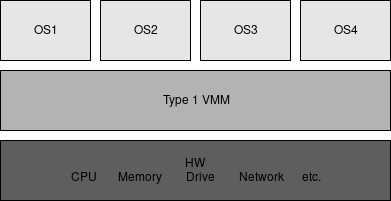
\includegraphics[width=0.65\textwidth]{png/VMMType1.png}
		\caption{Aufruf des FilterVIs}
		\label{fig:filterVI}
	\end{center}
\end{wrapfigure}
Ein Typ-1-Hypervisor (bare-matel oder auch native genannt) setzt direkt auf der Hardware auf. Es benötigt kein Betriebssystem, auf welchem dieses Läuft. Es wird jedoch vorausgesetzt, dass die Hardware des Hostsystems vom Typ-1-Hypervisor durch entsprechende Treiber unterstützt wird.\\

\newpage
\subsubsection{Type 2}
\begin{wrapfigure}{r}{0.73\textwidth}
	\begin{center}
		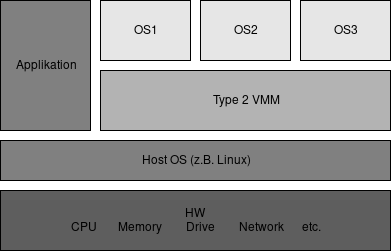
\includegraphics[width=0.6\textwidth]{png/VMMType2.png}
		\caption{Aufruf des asd}
		\label{fig:as}
	\end{center}
\end{wrapfigure}
Ein Typ-2-Hypervisor setzt auf einem vollwertigen Betriebssystem, welches auf dem Hostsystem installiert ist, auf und nutzt die Treiber, des Betriebssystemes, um auf die Hardwareresourcen des Hostsystemes zuzugreifen zu können. Dementsprechend sind alle Typ-2-Hypervisoren auf einem Hostsystem lauffähig, sofern sich auf diesem das unterstützte Hostbetriebssystem installieren lässt.
\section{KVM}
KVM steht für Kernel Based Virtualmachine. bei KVM handelt es sich um eine Infrastruktur des Linux-Kernels zur Virtualisirung. Die Virtualisierung auf verschiedenen Plattformen unterstützt, unter anderem die folgenden Intel, AMD, ARM, PowerPC und System Z. KVM selbst nimmt keine Emulation vor, es ist also nicht möglich eine Bestimmte hardware zu emulieren mit KVM selbst. so würde es sich als enorm Schwer erweisen ein vollwertiges Betriebssystem auf dem Hostsystem nur mit hilfe von KVM zu installieren. Um die Emulation zu ermöglichen hat sich QEMU als defacto standart etabliert. QEMU steht für Quick Emulator uns stellt für virtualisierte Gastsysteme die notwendigen Geräte wie Festplatten, Netwerk-, Sound- und Grafikkarten zur Verfügung.\\
KVM ist desweiteren auch eine Quellofene lösung, und ist neben XEN der Weitverbreiteste Quellofene Hypervisor. Trotz einigen aussagen ist KVM jedoch ein Type 2 Hypervisor und nicht wie XEN ein Type 1.

\subsection{Funktionsumfang}
KVM ist bereits bei der Installation eine sehr schlanke und einfache umgebung. 
Es sind im Wesentlichen nur die KVM Kernel Module dem bestehenden System dazuzuinstallieren sowie Qemu und Management-Tools einzurichten. Der Vorteil liegt hier auch, dass viele schon bestehende Linux-Server nachträglich zu einem Virtualisierungssystem aufgerüstet werden kann ohne damit eine Komplette neuinstallation tätigen zu müssen.
Weiter verhält sich jede  Virtuelle CPU (kurz VCPU) im Gastsystem wie ein gewöhnlicher Linux-Process und kann so beispielsweise auch üüber normale Kommandos wie kill oder top kontrolliert und gesteuert werden. Das selbe gilt auch für die Gerätelandschaft. Da mit KVM und Qemu die normalen Linux-Treiber genutzt werden können, ist eine Umgewühnung für einen Linux-Administrator nicht nötig.\\

KVM in zusammenarbeit mit Qemu unterstützt eine enorme anzahl an Gast-Betriebssysteme, darunter finden sich fast Sämtliche wichtigen Windows-Varianten sowie Linux, Solaris, BSD, FreeBSD und einige exotischere wie ReactOS.\\

Ein Nachteil der KVM ist jedoch, dass sie nicht auf Graphische Systeme ausgerichtet ist, es ist also die idee, dass ein Gastsystem, welches auf einer KVM instaz läuft, nur über ein Terminal bedient wird.\\
Beim Management zeigt sich, wie stark sich die Marktposition dieses Quelloffenen Open-Source-Hypervisors verbessert hat. Es ist inzwischen ein Fülle von Administrationswerkzeugen verfügbar, zudem wird KVM in vielen Cloud-Plattformen eingebaut.
Durch die simplen tools virt-manager sowie virsh ist schon eine Remote-Management möglich. Für vortgeschrittene Funktionen wie Orchestrierung ganzer Pools von Virtuellen Maschinen mit weitergehenden funktionen wie Failover, High Availability und dergleichen gibt es weitere Lösungen. Hier springen Drittobjekte sowie Softwarehersteller in dir Bresche, normalerweise auch Open Source. 

Es gibt zudem für auf KVM aufbauende Komplettlösungen für die Servervirtualisierung. allen voran RHEV (Red Hat Virtualization).
 
Für die Verwaltung der Gastsysteme gibt im Wesentlichen viele verschiedene Tools, von einfachen verwaltungssoftware für den Desktop PC wie zum Beispiel Gnome-Boxe
\subsection{KVM on System Z}
\begin{tabular}{ | l | c | r | } \hline
	Test1 & Test2 & Test3 \\ \hline
	TestA & TestB & TestB \\ \hline
\end{tabular}
http://www.redbooks.ibm.com/redbooks/pdfs/sg248332.pdf




\section{ESXi}
\subsection{Funktionsumfang}
\chapter{Vergleich}
\chapter{Fazit}
\chapter{Anhang}




\chapter{Wayne}
Ein vergleich im eigentlichen sinne stellt sich hier als enorm Schwierig dar. Da Zwei unterschiedliche einsatzgebiete miteinander verglichen werden sollen. Die Systeme, welche verglichen werden sollen, werden gemäs der Aufgabenstellung nicht einmal auf der Selben hardware verglichen sondern auf 2 für verschiedene Anwendungen gedachte lösungen. Der Auftrag an sich ist als ob ich eine Luxuskreuzfahrtschiff mit einem Transportschiff verglichen werden soll. So gibt es schon gemeinsamkeiten, jedoch kann kein wahrer, endgültiger und absoluter vergleich aufgestellt werden. Es kann auch kein wahrer gewinner aufgezeigt werden, da beide Lösungen in sich gut sind. Es soll mehr für den jeweiligen einsatzzweck sowie den gewünschten Funktionen einen individuellen entscheid getroffen werden. Ich möchte hiermit trozdem darlegen, welches die ungefähren unterschiede der beiden lösungen darstellt, damit eine Entscheidungsfindung unter umsten vereinfacht werden kann.



++
Wie man den vorangegangenen Kapitel nun entnehmne kann, sind beide Lösungsansätze eine gute wahl.
\footfullcite{website:hs-rm}


\chapter{Was ist Virtualisierung}
Unter der Virtualisiertung versteht man in der Informatik unter anderem die Technologie, bie welcher das Betriebssystem nicht unmittelbar auf einer Physischen Instanz wie einem Server, oder DesktopPCs installiert ist, sondern auf der Hardware über einer Zwischenschicht, welche die reale phyisische hardware abstrahiert, oder aber in einem Gastgeber-Betriebssystem mittels einer Viertualisierungssoftware wie VirtualBox.
Dieses auf der virtuellen umgebung laufende Betriebssystem nennt man Gastsysteme.
Die tatsächliche vorhandene Hardwareumgebung wird als Hostsystem bezeichnet. Die Softwareschicht, welche diese Gastsysteme verwaltet nennt man Hypervisor (Klassifikationen Siehe Kapitel XYZ).
Dieser Hypervisor verwaltet die Ressourcen und dessen zuteilung für die einzelnen Gastsysteme. Dabei verteilt der Hypervisor die Resourcen so, dass alle resourcen für das Gastsystem verfügbar sind, wenn dieses es benötigt, so als ob nur jenes Gastsystem vorhanden wäre.
Dem Gastsystem wird dank des Hypervisors eine eigener vollständiger Rechner vorgetäuscht, mit allen Hardwar-Elementen welche dazugehören. Das abstrahieren des Hypervisors und vortäuschen einer Realen hardware führt dazu, dass das Gastsystem nicht nur auf der Reellen hardware lauffähig ist in der es installiert wurde, sondern auf allen, in denen der Hypervisor installiert bzw. lauffähig ist.



++Kurze geschichte zur Virtualisierung
Die ersten Hypervisoren, die Virtualisierung ermgölichten, 



Unter Virtualisierung versteht man unter anderem eine Technologie, bei der eine Betriebssysteminstanz nicht unmittelbar auf einem Physischen Rechner, z.B Server, installiert ist, sondern auf der Hardwere über einer Zwischensicht, die von der Hardware abstrahiert, oder aber in einem Gastgeber-Betriebssystem mittels Virtualisierungssoftware, z.B. VMWare oder Virtual Box.

In der Informatik bezeichnet Virtualisierung das Nachbilden eines Hardware- Softwareobjektes, welches vom selben typ wie die tatsächliche darunterliegende Hardware/Software ist.
Dieses Nachbilden geschieht mit hilfe eines Abstraktionslayers.




\section{Grundlagen der Virtualisierung}


Die Geschichte der Virtualisierung liegt schon eine lange Zeit zurück. Bereits in den frühen 1960er Jahre hat IBM 








++Hypervisor klassifikationen.
Ein Hypervisor lässt sich typischer weise in einen von 2 Typen unterteilen.
+Typ1 Naitive or bare metal
Native Hypervisoren sind softwaresysteme, welche direkt auf der Hardware des Hostsystemes laufen um die Hardware zu kontrollieren und die Gastsysteme zu überwachen. . 


Diesens auf der abstrahierten, virtuellen umgebung laufende Betriebssystem nennt man Gastsystem.



\chapter{KVM}
Die Kernel-based Virtual Machine ist eine Virtualisierungslösung welche in den Linuxkernel integriert wurde. 

Die Kernel-based Virtual Machine ist eine Infrastruktur des Linux-Kernel zur Virtualisirung 


https://www.cs.hs-rm.de/~linn/fachsem0910/hirt/KVM.pdf
https://www.tecchannel.de/a/kostenlose-virtualisierungssoftware-im-vergleich,2051909,4
https://www.tecchannel.de/a/kostenlose-virtualisierungssoftware-im-vergleich,2051909,5

\printbibliography
\end{document}

